\section{Nuclear Elastic Differential Cross Sections}
The nuclear-elastic, interference, and nuclear-reaction differential cross sections do not have analytical forms, and are instead tabulated in data sets. In this work the LANL charged particle data sets are used, which are tabulated in the evaluated nuclear data format (ENDF) files \cite{Brown-2018}. The LANL charged particle data sets were selected because they contain interference differential cross sections that are evaluated over the full angular range and are not cut off when the interference differential cross section becomes negative \cite{Perkins-1981} \cite{Hale-1983}. In the ENDF files, the NES and nuclear-reaction differential cross sections are tabulated in terms of Legendre expansions as
\begin{equation} \label{eqn:nes_differential cross section}
    \sigma_{x,t \rightarrow x}^N(E^{\prime} \rightarrow E; \mucm) = \sum_{l=0}^L \dfrac{2l+1}{2} b_l(E^{\prime}) P_l(\mucm),
\end{equation}
and
\begin{equation}\label{eqn:nuclear-reaction_differential cross section}
    \sigma_{x,t \rightarrow s}(E^{\prime} \rightarrow E; \mucm) = \dfrac{1}{2} + \sum_{l=1}^N \dfrac{2l+1}{2} b_l(E^{\prime}) P_l(\mucm),
\end{equation}
where $P_l(\mucm)$ are the Legendre polynomials of order $l$, and $b_l(E)$ are the tabulated Legendre expansion coefficients. Similarly, the interference differential cross sections are expressed in the ENDF files in terms of a complex Legendre expansion as,
\begin{equation} \label{eqn:interference_differential cross section}
    \sigma_{x,t \rightarrow x}^I(E^{\prime} \rightarrow E; \mucm) = -\dfrac{2 \eta(E^{\prime})}{1 - \mucm} \text{Re} \left\lbrace \text{exp}\left[ i \eta(E^{\prime}) \text{ln}\left(\frac{1 - \mucm}{2} \right)\right] \sum_{l=0}^L \dfrac{2l+1}{2} a_l(E) P_l(\mucm) \right\rbrace,
\end{equation}
where $\eta(E)$ is the dimensionless Coulomb parameter given in Eq.~\eqref{eqn:Coulomb_parameters}, and $a_l(E)$ are the complex Legendre coefficients.

Figure \ref{fig:sig_n} shows a plot of the NES differential cross section for energetic deuterons colliding with tritons at various incident energies. From Figure \ref{fig:sig_n}, it can be concluded that at low incident ion energies NES is not an important collision effect, but as the incident energy of the particle increases NES collisions become important. Additionally, the NES differential cross sections allow for back-scattering collisions to occur when the incident energies of the ions are high enough. These back-scatter collisions produce energetic recoil ions that have been shown to be an important effect in the heating of the plasma \cite{Nakao-1988}. In general, it can be concluded that NES collisions are not highly peaked and that they have large MFPs when compared to the corresponding Coulomb differential cross sections.

\begin{figure}[!htb]
    \centering
    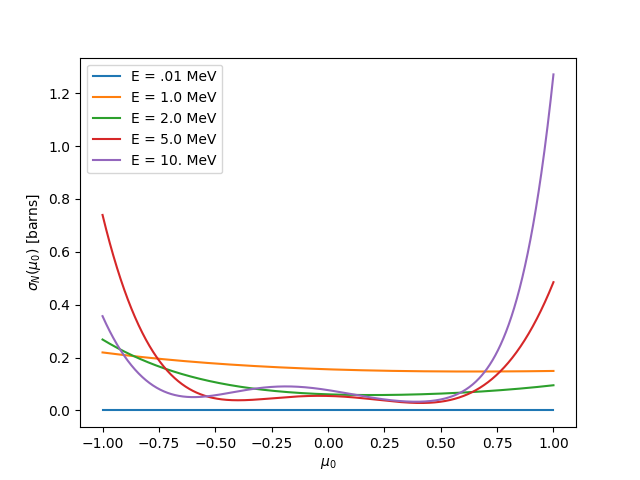
\includegraphics[scale=0.75]{../figures/proposed_work/sig_n_dt.png}
    \caption{Nuclear-elastic scattering differential cross section for deuterons colliding with tritons at 1.0 MeV}
    \label{fig:sig_n}
\end{figure}